\documentclass[11pt]{article}

\usepackage[a4paper,margin=0.75in]{geometry}
\usepackage{amsmath,amssymb}
\usepackage{graphicx}
\usepackage{booktabs}
\usepackage{array}
\usepackage{float}
\usepackage{hyperref}
\usepackage{enumitem}
\usepackage{xcolor}
\usepackage{tikz}
\usetikzlibrary{positioning,arrows.meta,shapes.geometric}

\setlist{nosep}
\renewcommand{\arraystretch}{1.3}

\tikzset{
layer/.style={
draw,
rounded corners,
minimum width=2.2cm,
minimum height=0.9cm,
align=center,
fill=blue!10
},
arrow/.style={
-{Latex[length=3mm]},
thick
}
}

\begin{document}

%%%%%%%%%%%%%%%%%%%%%%%%%%%%%%%%%%%%%%%%%%%%%%%%%%%%%%%%%%%%

\begin{center}

{\Large\textbf{Shiv Nadar University Chennai}}

\vspace{3mm}

{\large\textbf{CS3807 -- Deep Learning Laboratory}}

\vspace{3mm}

{\Large\textbf{Experiment 4}}

\vspace{2mm}

{\Large\textbf{Comparative Study of Deep Convolutional Neural}}

{\Large\textbf{Network Architectures Using Transfer Learning}}

\end{center}

\vspace{5mm}

\begin{tabular}{|p{4cm}|p{8cm}|p{2cm}|}
\hline
Degree \& Branch &
B.Tech Artificial Intelligence \& Data Science &
Semester V\\
\hline
Subject Code \& Name &
CS3807 -- Deep Learning Laboratory &
AY: 2026--27\\
\hline
\end{tabular}

%%%%%%%%%%%%%%%%%%%%%%%%%%%%%%%%%%%%%%%%%%%%%%%%%%%%%%%%%%%%

\section*{1. Objective}

The objectives of this experiment are

\begin{itemize}

\item Study the evolution of deep CNN architectures.

\item Compare LeNet-5, AlexNet, VGG16, GoogleNet and ResNet.

\item Understand transfer learning.

\item Fine tune pretrained CNN models.

\item Compare classification performance of different architectures.

\end{itemize}

%%%%%%%%%%%%%%%%%%%%%%%%%%%%%%%%%%%%%%%%%%%%%%%%%%%%%%%%%%%%

\section*{2. Learning Outcomes}

After completing this experiment students will be able to

\begin{enumerate}

\item Explain modern CNN architectures.

\item Differentiate LeNet, AlexNet, VGG16, GoogleNet and ResNet.

\item Implement transfer learning.

\item Fine tune pretrained CNN models.

\item Compare CNN architectures using performance metrics.

\end{enumerate}

%%%%%%%%%%%%%%%%%%%%%%%%%%%%%%%%%%%%%%%%%%%%%%%%%%%%%%%%%%%%

\section*{3. Introduction}

Deep Convolutional Neural Networks have become the dominant models for
computer vision applications because they automatically learn hierarchical
features from images. The evolution of CNNs has focused on improving
classification accuracy while reducing computational complexity and
training difficulties.

The progression of CNN architectures began with LeNet-5 and has evolved
through AlexNet, VGGNet, GoogleNet, and ResNet. Each architecture
introduced important innovations that significantly improved image
classification performance.

%%%%%%%%%%%%%%%%%%%%%%%%%%%%%%%%%%%%%%%%%%%%%%%%%%%%%%%%%%%%

\section*{4. Evolution of CNN Architectures}

\begin{center}

\begin{tabular}{|c|c|p{7cm}|}

\hline

Model & Year & Major Contribution\\

\hline

LeNet-5 & 1998 &
First practical convolutional neural network\\

\hline

AlexNet & 2012 &
ReLU activation, Dropout and GPU training\\

\hline

VGG16 & 2014 &
Uniform $3\times3$ convolution filters\\

\hline

GoogleNet & 2014 &
Inception modules for multi-scale feature extraction\\

\hline

ResNet & 2015 &
Residual learning using skip connections\\

\hline

\end{tabular}

\end{center}

%%%%%%%%%%%%%%%%%%%%%%%%%%%%%%%%%%%%%%%%%%%%%%%%%%%%%%%%%%%%

\section*{5. LeNet-5}

LeNet-5 was proposed by Yann LeCun in 1998 for handwritten digit
recognition. It consists of two convolution layers, two average pooling
layers and fully connected layers. It demonstrated that convolutional
networks could automatically learn image features without handcrafted
feature extraction.


Advantages

\begin{itemize}

\item Small number of parameters

\item Fast training

\item Suitable for OCR

\end{itemize}

%%%%%%%%%%%%%%%%%%%%%%%%%%%%%%%%%%%%%%%%%%%%%%%%%%%%%%%%%%%%

\section*{6. AlexNet}

AlexNet won the ImageNet Challenge in 2012 by reducing the
classification error significantly. It introduced ReLU activation,
Dropout regularization and GPU training.


Major innovations

\begin{itemize}

\item ReLU activation

\item Dropout

\item GPU implementation

\item Data augmentation

\end{itemize}

%%%%%%%%%%%%%%%%%%%%%%%%%%%%%%%%%%%%%%%%%%%%%%%%%%%%%%%%%%%%

\section*{7. VGG16}

VGG16 demonstrated that using multiple small $3\times3$ convolution
filters could outperform larger filters while increasing network depth.


Advantages

\begin{itemize}

\item Excellent feature extraction

\item Simple architecture

\item High classification accuracy

\end{itemize}

%%%%%%%%%%%%%%%%%%%%%%%%%%%%%%%%%%%%%%%%%%%%%%%%%%%%%%%%%%%%

\section*{8. Comparison of Architectures}

\begin{center}

\begin{tabular}{|l|c|c|c|}

\hline

Architecture &
Depth &
Parameters &
Main Contribution\\

\hline

LeNet-5 &
7 &
60K &
First CNN\\

AlexNet &
8 &
61M &
ReLU + Dropout\\

VGG16 &
16 &
138M &
Deep 3$\times3$ filters\\

GoogleNet &
22 &
6.8M &
Inception Modules\\

ResNet50 &
50 &
25.6M &
Residual Learning\\

\hline

\end{tabular}

\end{center}

% --------- CONTINUE WITH PART 2 ---------
%%%%%%%%%%%%%%%%%%%%%%%%%%%%%%%%%%%%%%%%%%%%%%%%%%%%%%%%%%%%
\section*{9. GoogleNet (Inception Network)}

GoogleNet, proposed by Szegedy \textit{et al.} in 2014, introduced the
\textbf{Inception Module}, which performs multiple convolution operations
in parallel using different filter sizes. Instead of using only a single
kernel size, GoogleNet simultaneously applies $1\times1$, $3\times3$,
$5\times5$ convolutions and max pooling. The outputs are concatenated to
obtain multi-scale feature representations.

The use of $1\times1$ convolutions before larger kernels reduces the
number of trainable parameters and computational complexity.


Advantages

\begin{itemize}
\item Multi-scale feature extraction.
\item Fewer parameters than VGG16.
\item High computational efficiency.
\item Better classification performance.
\end{itemize}

%%%%%%%%%%%%%%%%%%%%%%%%%%%%%%%%%%%%%%%%%%%%%%%%%%%%%%%%%%%%

\section*{10. ResNet}

Increasing CNN depth often causes the \textbf{vanishing gradient problem},
making optimization difficult. ResNet solves this issue using
\textbf{skip (residual) connections}, allowing gradients to flow directly
through the network.

Instead of learning

\[
H(x)
\]

ResNet learns

\[
F(x)=H(x)-x
\]

thus,

\[
Output = F(x)+x
\]

where

\begin{itemize}
\item $F(x)$ = Residual Mapping
\item $x$ = Identity Mapping
\end{itemize}

\begin{figure}[H]
\centering

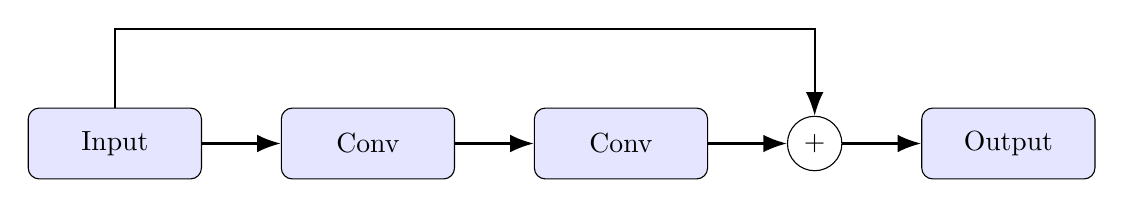
\begin{tikzpicture}[node distance=1cm]

\node[layer](input){Input};

\node[layer,right=of input](conv1){Conv};

\node[layer,right=of conv1](conv2){Conv};

\node[circle,draw,right=of conv2](add){+};

\node[layer,right=of add](output){Output};

\draw[arrow](input)--(conv1);
\draw[arrow](conv1)--(conv2);
\draw[arrow](conv2)--(add);
\draw[arrow](add)--(output);

\draw[arrow]
(input)
|-([yshift=10mm]conv2.north)
-| (add.north);

\end{tikzpicture}

\caption{Residual Block in ResNet}
\end{figure}

Advantages

\begin{itemize}
\item Eliminates vanishing gradients.
\item Enables very deep neural networks.
\item Faster convergence.
\item High ImageNet accuracy.
\end{itemize}

%%%%%%%%%%%%%%%%%%%%%%%%%%%%%%%%%%%%%%%%%%%%%%%%%%%%%%%%%%%%

\section*{11. Dilated Convolution}

Dilated convolution (also called atrous convolution) increases the
receptive field without increasing the number of parameters.

The dilation rate determines the spacing between kernel elements.

For a standard convolution,

\[
D=1
\]

For dilated convolution,

\[
D>1
\]

Example

\[
\begin{bmatrix}
1 & 0 & 2\\
0 & 3 & 0\\
4 & 0 & 5
\end{bmatrix}
\]

where zeros indicate inserted gaps.

Applications

\begin{itemize}
\item Semantic segmentation
\item Medical image analysis
\item Satellite imagery
\item Object localization
\end{itemize}

%%%%%%%%%%%%%%%%%%%%%%%%%%%%%%%%%%%%%%%%%%%%%%%%%%%%%%%%%%%%

\section*{12. Transpose Convolution}

Transpose convolution increases the spatial dimensions of feature maps.
Unlike pooling, which reduces image size, transpose convolution performs
learnable upsampling.

Applications

\begin{itemize}
\item Image Super Resolution
\item Autoencoders
\item GANs
\item Image Generation
\item Semantic Segmentation
\end{itemize}

%%%%%%%%%%%%%%%%%%%%%%%%%%%%%%%%%%%%%%%%%%%%%%%%%%%%%%%%%%%%

\section*{13. Transfer Learning}

Transfer Learning utilizes a pretrained CNN model that has already learned
general image features from a large dataset such as ImageNet.

Instead of training from scratch,

\begin{enumerate}
\item Load a pretrained model.
\item Remove the original classifier.
\item Freeze convolution layers.
\item Add new Dense layers.
\item Train the classifier.
\item Fine tune selected convolution layers.
\end{enumerate}

\begin{figure}[H]

\centering

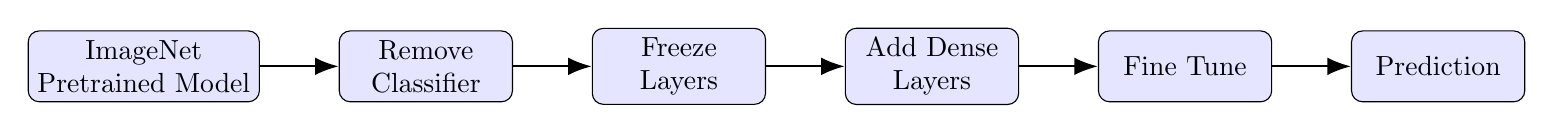
\begin{tikzpicture}[node distance=1cm]

\node[layer](a){ImageNet\\Pretrained Model};

\node[layer,right=of a](b){Remove\\Classifier};

\node[layer,right=of b](c){Freeze\\Layers};

\node[layer,right=of c](d){Add Dense\\Layers};

\node[layer,right=of d](e){Fine Tune};

\node[layer,right=of e](f){Prediction};

\foreach \x/\y in {a/b,b/c,c/d,d/e,e/f}
\draw[arrow](\x)--(\y);

\end{tikzpicture}

\caption{Transfer Learning Workflow}

\end{figure}

Advantages

\begin{itemize}
\item Faster convergence.
\item Higher accuracy on small datasets.
\item Reduced training time.
\item Lower computational cost.
\end{itemize}

%%%%%%%%%%%%%%%%%%%%%%%%%%%%%%%%%%%%%%%%%%%%%%%%%%%%%%%%%%%%

\section*{14. Dataset}

Dataset: CIFAR-10

\begin{itemize}

\item Training Images : 50,000

\item Testing Images : 10,000

\item Number of Classes : 10

\item Image Size : $32\times32\times3$

\item Classes:
Airplane, Automobile, Bird, Cat, Deer,
Dog, Frog, Horse, Ship and Truck.

\end{itemize}

%%%%%%%%%%%%%%%%%%%%%%%%%%%%%%%%%%%%%%%%%%%%%%%%%%%%%%%%%%%%
% Continue with Part 3
%%%%%%%%%%%%%%%%%%%%%%%%%%%%%%%%%%%%%%%%%%%%%%%%%%%%%%%%%%%%

\section*{15. Experimental Procedure}

\subsection*{Task 1: Dataset Preparation}

\begin{enumerate}

\item Load the CIFAR-10 dataset using TensorFlow/Keras.

\item Normalize the pixel values to the range [0,1].

\item Display ten sample images.

\item Print the dimensions of the training and testing datasets.

\end{enumerate}

%%%%%%%%%%%%%%%%%%%%%%%%%%%%%%%%%%%%%%%%%%%%%%%%%%%%%%%%%%%%

\subsection*{Task 2: Transfer Learning}

Load any one of the following pretrained CNN models.

\begin{itemize}

\item VGG16

\item ResNet50

\item MobileNetV2

\item EfficientNetB0 (Optional)

\end{itemize}

Perform the following steps.

\begin{enumerate}

\item Load pretrained ImageNet weights.

\item Remove the original classification layer.

\item Freeze the convolutional base.

\item Add a Global Average Pooling layer.

\item Add a Dense layer with ReLU activation.

\item Add the output layer with Softmax activation.

\end{enumerate}

%%%%%%%%%%%%%%%%%%%%%%%%%%%%%%%%%%%%%%%%%%%%%%%%%%%%%%%%%%%%

\subsection*{Task 3: Model Training}

Train the model using

\begin{center}

\begin{tabular}{|p{5cm}|p{6cm}|}

\hline

Optimizer & Adam\\

\hline

Learning Rate & 0.001\\

\hline

Batch Size & 32\\

\hline

Epochs & 10--20\\

\hline

Loss Function &
Categorical Cross Entropy\\

\hline

Evaluation Metric &
Accuracy\\

\hline

\end{tabular}

\end{center}

%%%%%%%%%%%%%%%%%%%%%%%%%%%%%%%%%%%%%%%%%%%%%%%%%%%%%%%%%%%%

\subsection*{Task 4: Fine Tuning}

\begin{enumerate}

\item Unfreeze the last convolution block.

\item Train for another 5--10 epochs.

\item Compare the classification accuracy before and after fine tuning.

\end{enumerate}

%%%%%%%%%%%%%%%%%%%%%%%%%%%%%%%%%%%%%%%%%%%%%%%%%%%%%%%%%%%%

\subsection*{Task 5: Model Evaluation}

Evaluate the trained model using

\begin{itemize}

\item Accuracy

\item Precision

\item Recall

\item F1-score

\item Confusion Matrix

\item Classification Report

\end{itemize}

%%%%%%%%%%%%%%%%%%%%%%%%%%%%%%%%%%%%%%%%%%%%%%%%%%%%%%%%%%%%

\section*{16. Hyperparameter Study}

Compare the performance using different settings.

\begin{center}

\begin{tabular}{|l|l|}

\hline

Hyperparameter & Values\\

\hline

Learning Rate &
0.001, 0.0001\\

\hline

Batch Size &
16, 32, 64\\

\hline

Epochs &
10, 20\\

\hline

Optimizer &
Adam, SGD\\

\hline

Dense Units &
128, 256\\

\hline

Frozen Layers &
All, Partial\\

\hline

\end{tabular}

\end{center}

%%%%%%%%%%%%%%%%%%%%%%%%%%%%%%%%%%%%%%%%%%%%%%%%%%%%%%%%%%%%

\section*{17. Source Code}


The complete source code, datasets, generated plots, and report files for this experiment are available in the following GitHub repository:



\noindent\textbf{GitHub Repository:} \\
\url{https://github.com/VIKASNI-S/Deep-Learning-Lab/tree/main/Lab-4}\\


\section*{18. Mandatory Plots}

\begin{enumerate}

\item Sample CIFAR-10 images

\begin{figure}[H]
\centering
\includegraphics[width=0.8\linewidth]{01_sample_cifar10.eps}

\label{fig:sampleimage}
\end{figure}
The figure shows representative images from the CIFAR-10 dataset belonging to different classes such as airplane, automobile, bird, cat, and dog.
The images demonstrate the diversity of objects used for training and evaluating the VGG16 transfer-learning model.
\vspace{0.5cm}

\item Training Accuracy

\begin{figure}[H]
    \centering
    \includegraphics[width=0.8\linewidth]{02_training_accuracy.eps}
    \label{fig:trainingaccuracy}
\end{figure}

Training accuracy increases progressively across the epochs, indicating that the VGG16 model learns useful features from the CIFAR-10 training data.
The final training accuracy is 97.98\%.

\vspace{0.5cm}



\item Validation Accuracy

\begin{figure}[H]
\centering
\includegraphics[width=0.8\linewidth]{03_validation_accuracy.eps}

\label{validationaccuracy}
\end{figure}
Validation accuracy improves during training, showing that the learned features generalize to unseen validation images.
The difference between the high training accuracy and validation accuracy indicates some degree of overfitting.
\vspace{0.5cm}

\item Training Loss

\begin{figure}[H]
\centering
\includegraphics[width=0.8\linewidth]{04_training_loss.eps}

\label{fig:trainingloss}
\end{figure}
Training loss decreases as the number of epochs increases, indicating that the model's prediction error is reducing during training.
The decreasing loss confirms that the model is effectively learning the CIFAR-10 training patterns.
\vspace{0.5cm}


\item Validation Loss
\begin{figure}[H]
\centering
\includegraphics[width=0.8\linewidth]{05_validation_loss.eps}

\label{fig:validationloss}
\end{figure}
% The model accuracy varies with different hyperparameter settings, demonstrating that hyperparameter selection significantly influences CNN performance. The optimal combination of learning rate, batch size, optimizer, and number of epochs achieved the highest classification accuracy.
Validation loss generally decreases as the model learns, indicating improved performance on unseen data.
If the validation loss begins to increase while training loss continues to decrease, it indicates overfitting to the training dataset.
\vspace{0.5cm}
\vspace{0.5cm}
\vspace{0.5cm}
\vspace{0.5cm}
\vspace{0.5cm}


\item Confusion Matrix

\begin{figure}[H]
\centering
\includegraphics[width=0.8\linewidth]{06_confusion_matrix.eps}

\label{fig:confusionmatrix}
\end{figure}
The confusion matrix shows the distribution of correct and incorrect predictions across the ten CIFAR-10 classes.
Classes such as Automobile, Frog, Horse, Ship, and Truck show relatively strong classification performance, while Cat and Dog have more confusion with other classes.
\vspace{0.5cm}

\item Misclassified Images (Optional)

\begin{figure}[H]
\centering
\includegraphics[width=0.8\linewidth]{07_misclassified_images.eps}

\label{fig:misclassifiedimages}
\end{figure}
The misclassified images show examples where the VGG16 model predicts a class different from the actual class.
These errors are expected because CIFAR-10 images have a low resolution of 32×32 pixels, making visually similar classes more difficult to distinguish.
\vspace{0.5cm}



\item Training Time Comparsion
\begin{figure}[H]
    \centering
    \includegraphics[width=0.85\textwidth]{07_training_time_comparison.eps}


    \caption{Training Time Comparison of CNN Architectures}
    \label{fig:training_time_comparison}
\end{figure}
ResNet50 achieved a good balance between training time and performance, taking 989.02 seconds.
VGG16 required the highest training time of 2412.28 seconds, while LeNet-5 was the fastest at 50.82 seconds.
GoogleNet trained considerably faster than AlexNet and VGG16, with a training time of 369.05 seconds.
\vspace{0.5cm}

\item Accuracy Comparsion
\begin{figure}[H]
    \centering
    \includegraphics[width=0.85\textwidth]{06_accuracy_comparison.eps}
    \caption{Accuracy Comparison of CNN Architectures}
    \label{fig:accuracy_comparison}
\end{figure}
ResNet50 achieved the highest accuracy of 81.33%, followed by VGG16 with 77.60%.
GoogleNet achieved a moderate accuracy of 65.13%, while LeNet-5 and AlexNet achieved 42.20% and 30.93%, respectively.
Overall, ResNet50 provided the best classification performance among the architectures evaluated.
\vspace{0.5cm}
\end{enumerate}

%%%%%%%%%%%%%%%%%%%%%%%%%%%%%%%%%%%%%%%%%%%%%%%%%%%%%%%%%%%%

\section*{19. Results}

\subsection*{19.1 Performance Metrics}

\begin{center}

\begin{tabular}{|p{5cm}|p{4cm}|}
\hline
\textbf{Metric} & \textbf{Value} \\
\hline
Training Accuracy & 0.9798 \\
\hline
Testing Accuracy & 0.7770 \\
\hline
Precision & 0.7783 \\
\hline
Recall & 0.7770 \\
\hline
F1-score & 0.7773 \\
\hline
Training Time & 4428.18 seconds \\
\hline
Total Parameters & 14,781,642 \\
\hline
\end{tabular}

\end{center}

\vspace{5mm}

\subsection*{19.2 Comparison of CNN Architectures}

\begin{center}
\begin{tabular}{|l|c|c|c|}
\hline
\textbf{Model} & \textbf{Parameters} & \textbf{Accuracy (\%)} & \textbf{Training Time (s)} \\
\hline
LeNet-5 & 83,126 & 42.20 & 50.82 \\
\hline
AlexNet & 21,557,642 & 30.93 & 1985.30 \\
\hline
VGG16 & 14,781,642 & 77.60 & 2412.28 \\
\hline
GoogleNet (InceptionV3) & 22,066,346 & 65.13 & 369.05 \\
\hline
ResNet50 & 23,851,274 & 81.33 & 989.02 \\
\hline
\end{tabular}
\end{center}

%%%%%%%%%%%%%%%%%%%%%%%%%%%%%%%%%%%%%%%%%%%%%%%%%%%%%%%%%%%%

% \section*{20. Discussion Questions}

% Answer the following questions.

% \begin{enumerate}

% \item Why is AlexNet considered a breakthrough in deep learning?

% \item Why does VGG16 use only $3\times3$ convolution filters?

% \item Explain the advantages of the Inception module.

% \item What is the purpose of residual learning?

% \item Differentiate LeNet and ResNet.

% \item What is Transfer Learning?

% \item Why is fine tuning required?

% \item Explain the difference between dilated convolution and transpose convolution.

% \item Why do pretrained models converge faster?

% \item Compare the computational complexity of LeNet and ResNet.

% \end{enumerate}


\section*{20. Discussion Questions}

\begin{enumerate}

\item \textbf{Why is AlexNet considered a breakthrough in deep learning?}

AlexNet was a major breakthrough because it showed that a deep convolutional neural network could achieve very high accuracy on large-scale image classification tasks. It made effective use of GPUs for faster training and introduced techniques such as ReLU activation and dropout. Its success on the ImageNet dataset played an important role in bringing deep learning into mainstream computer vision.

\vspace{5mm}
\item \textbf{Why does VGG16 use only $3\times3$ convolution filters?}

VGG16 mainly uses small $3\times3$ filters because they can capture useful local features while keeping the number of parameters relatively low. Multiple $3\times3$ convolution layers can also provide a larger effective receptive field while adding more nonlinear activation layers. This allows the network to learn complex features without using very large filters.

\vspace{5mm}
\item \textbf{Explain the advantages of the Inception module.}

The Inception module allows the network to process an image using different filter sizes at the same time. This helps the model capture both small and large patterns present in an image. It also uses $1\times1$ convolutions to reduce the number of channels, which helps control the computational cost and makes the network more efficient.
\vspace{5mm}
\item \textbf{What is the purpose of residual learning?}

Residual learning was introduced to make it easier to train very deep neural networks. Instead of directly learning the complete mapping, the network learns the difference, or residual, between the input and the desired output. Skip connections allow the input to bypass some layers, which helps reduce the vanishing gradient problem and makes deeper networks easier to optimize.
\vspace{5mm}
\item \textbf{Differentiate LeNet and ResNet.}

LeNet is an early and relatively simple CNN designed mainly for handwritten digit recognition. It contains only a few convolutional and pooling layers and has a small number of parameters. ResNet is much deeper and uses residual or skip connections, allowing it to train effectively even with many layers. Therefore, ResNet is more suitable for complex and large-scale image classification tasks.
\vspace{5mm}
\item \textbf{What is Transfer Learning?}

Transfer learning is the process of using a model that has already been trained on a large dataset and adapting it to a new task. Instead of training a CNN completely from scratch, the pretrained model can be used as a starting point. This is especially useful when the new dataset is relatively small, as the model already contains useful features such as edges, shapes, and textures.
\vspace{5mm}
\item \textbf{Why is fine tuning required?}

Fine tuning is used to adapt a pretrained model more closely to the new dataset and task. The pretrained layers already contain general image features, but the new dataset may have different characteristics. By training some of the later layers, and sometimes the earlier layers with a smaller learning rate, the model can learn features that are more specific to the new problem.
\vspace{5mm}
\item \textbf{Explain the difference between dilated convolution and transpose convolution.}

Dilated convolution increases the receptive field by inserting gaps between the elements of a convolution filter without increasing the number of filter parameters significantly. It is useful when we want to capture information from a larger area of an image while maintaining the spatial resolution. Transpose convolution, on the other hand, is mainly used to increase the spatial dimensions of feature maps and is commonly used in image generation and segmentation tasks.
\vspace{5mm}
\item \textbf{Why do pretrained models converge faster?}

Pretrained models converge faster because they do not start with completely random weights. They have already learned useful visual features such as edges, textures, shapes, and patterns from a large dataset. Therefore, when the model is trained on a new dataset, it only needs to adjust these existing features rather than learning everything from the beginning.
\vspace{5mm}
\item \textbf{Compare the computational complexity of LeNet and ResNet.}

LeNet has a relatively small number of layers and parameters, so it requires much less computation and memory during training and inference. ResNet is significantly deeper and contains millions of parameters, making it computationally more expensive. However, the residual connections in ResNet make it possible to train such deep networks effectively and achieve much better performance on complex image classification tasks.
\vspace{5mm}
\end{enumerate}
%%%%%%%%%%%%%%%%%%%%%%%%%%%%%%%%%%%%%%%%%%%%%%%%%%%%%%%%%%%%

\section*{21. Additional Exercises}

\begin{enumerate}

\item Implement transfer learning using VGG16.

\item Repeat the experiment using ResNet50.

\item Compare Adam and SGD optimizers.

\item Compare training with frozen layers and fine tuning.

\item Evaluate the model using Precision, Recall and F1-score.

\item Compare the performance of LeNet, AlexNet and ResNet.

\end{enumerate}

%%%%%%%%%%%%%%%%%%%%%%%%%%%%%%%%%%%%%%%%%%%%%%%%%%%%%%%%%%%%

\section*{22. References}

\begin{enumerate}

\item Yann LeCun, Leon Bottou, Yoshua Bengio and Patrick Haffner,
\emph{Gradient-Based Learning Applied to Document Recognition},
Proceedings of the IEEE, 1998.

\item Alex Krizhevsky, Ilya Sutskever and Geoffrey Hinton,
\emph{ImageNet Classification with Deep Convolutional Neural Networks},
NeurIPS, 2012.

\item Karen Simonyan and Andrew Zisserman,
\emph{Very Deep Convolutional Networks for Large-Scale Image Recognition},
ICLR, 2015.

\item Christian Szegedy et al.,
\emph{Going Deeper with Convolutions},
CVPR, 2015.

\item Kaiming He, Xiangyu Zhang, Shaoqing Ren and Jian Sun,
\emph{Deep Residual Learning for Image Recognition},
CVPR, 2016.

\item Ian Goodfellow, Yoshua Bengio and Aaron Courville,
\emph{Deep Learning},
MIT Press, 2016.

\item TensorFlow Documentation:
\url{https://www.tensorflow.org}

\item Keras Documentation:
\url{https://keras.io}

\end{enumerate}

%%%%%%%%%%%%%%%%%%%%%%%%%%%%%%%%%%%%%%%%%%%%%%%%%%%%%%%%%%%%

\end{document}